%% ===============================================================
\section{Methodology}
\label{sec:methodology}

\subsection{Problem Formulation}

Given a video $V = \{f_1, f_2, \ldots, f_N\}$ with $N$ frames, we seek a subset $S \subset V$ with $|S| = k \ll N$ that maximizes information retention $\mathcal{I}(S)$ subject to a cost constraint $C(S) \leq C_{\max}$:
\begin{equation}
\label{eq:optimization}
\max_{S \subset V} \; \mathcal{I}(S) \quad \text{s.t.} \quad |S| \cdot c_{\text{VLM}} \leq C_{\max}
\end{equation}
where $c_{\text{VLM}}$ is the per-frame VLM inference cost. Traditional approaches fix $k$ heuristically (e.g., $k = N/30$ for 1 FPS). We instead derive $k$ from video content properties.

\subsection{Adaptive Information Budgeting}
\label{sec:budget}

We define \textbf{Semantic Energy} $E_S$ for a video, inspired by the Hamiltonian $H = T + V$ where kinetic and potential energy jointly determine system behavior:
\begin{equation}
\label{eq:semantic_energy}
E_S = \underbrace{\bar{v}}_{\text{Semantic Velocity}} \cdot \underbrace{\bar{\mathcal{A}}}_{\text{Attention Yield}}
\end{equation}
where $\bar{v} = \text{mean}_t \|\phi(f_{t+1}) - \phi(f_t)\|_2$ is the mean CLIP embedding distance between consecutive frames (capturing temporal change rate), and $\bar{\mathcal{A}}$ is the mean Attention Yield across candidate frames:
\begin{equation}
\label{eq:attention_yield}
\mathcal{A}(f_t) = \alpha \cdot \text{TextPresence}(f_t) + \beta \cdot \text{FacePresence}(f_t) + \gamma \cdot \text{PositionalWeight}(f_t)
\end{equation}
with $\alpha = 0.4$, $\beta = 0.35$, $\gamma = 0.25$ tuned via grid search on 50 held-out ads. Text and face presence are detected via Tesseract OCR and a face detector respectively; positional weight boosts opening (1.5$\times$) and closing (1.4$\times$) segments where brand reveals and CTAs typically appear.

The \textbf{Intrinsic Semantic Dimensionality (ISD)} captures the effective rank of semantic variation:
\begin{equation}
\label{eq:isd}
k^* = \text{ISD}(V) = \min\left\{k : \frac{\sum_{i=1}^k \sigma_i^2}{\sum_{j=1}^N \sigma_j^2} \geq \tau\right\}
\end{equation}
where $\sigma_i$ are singular values from SVD of the centered CLIP embedding matrix $\Phi = [\phi(f_1), \ldots, \phi(f_N)]^\top$ and $\tau = 0.90$.

The final frame budget combines both quantities:
\begin{equation}
\label{eq:budget}
\text{budget} = \min\!\left(\text{base} + \lfloor 1.5 \cdot k^* \rfloor,\; \max\!\left(\text{base},\; \lfloor \text{base} + d \cdot \rho \cdot E_S \rfloor\right)\right)
\end{equation}
where $\text{base} = \max(5, |\text{scenes}| + 1)$ is a coverage floor, $d$ is video duration, and $\rho = 0.25$ is the base density. The ISD term caps the budget: semantically simple videos (low $k^*$) receive tight budgets (5--8 frames), while complex videos dynamically expand (30--50 frames). The Semantic Energy term scales the raw budget based on how rapidly and information-densely the video content changes.

%% Table and discussion of budget ablation are located in Section 6.1



\begin{figure*}[t]
\centering
%% figures/architecture.tex
%% Usage: %% figures/architecture.tex
%% Usage: %% figures/architecture.tex
%% Usage: \input{figures/architecture}  inside a figure* in main.tex
%%
%% Required in main.tex preamble:
%%   \usepackage{tikz}
%%   \usepackage{amsmath}
%%   \usetikzlibrary{positioning, shapes.geometric, shapes.symbols,
%%                   shadows, arrows.meta, fit, calc}

\resizebox{\textwidth}{!}{%
\begin{tikzpicture}[
    node distance=0.5cm and 0.8cm,
    >=Latex,
    font=\sffamily\scriptsize,
    %%
    box/.style={
        draw, rounded corners, align=center,
        minimum height=0.75cm, minimum width=1.6cm,
        fill=white, drop shadow
    },
    process/.style={box, fill=blue!5},
    decision/.style={
        draw, diamond, aspect=2.2,
        align=center, inner sep=1.5pt,
        minimum width=3.0cm, minimum height=0.85cm,
        fill=yellow!8, drop shadow,
        font=\sffamily\scriptsize
    },
    data/.style={
        draw, cylinder, shape border rotate=90, aspect=0.25,
        align=center, minimum height=1.0cm, minimum width=1.5cm,
        fill=gray!6, drop shadow,
        font=\sffamily\scriptsize
    },
    group/.style={
        draw=gray!60, dashed, rounded corners=4pt, inner sep=0.40cm,
        label={[anchor=north west, font=\sffamily\bfseries\scriptsize,
                text=gray!80, yshift=-0.05cm]north west:#1}
    },
    arrow/.style={->, thick, gray!60},
    highlight/.style={->, thick, blue!60!black},
    annotlabel/.style={font=\sffamily\tiny\bfseries, blue!70!black}
]

%% ── Input ────────────────────────────────────────────────────────────────────
\node[data] (input) {Video Input\\(AdBench-500)};

%% ── Frame Extraction ─────────────────────────────────────────────────────────
\node[process, right=1.0cm of input] (extract)
    {Frame Extraction\\\tiny 30\,FPS $\to$ $N$ frames};
\draw[highlight] (input) -- (extract);

%% ── Cascade stages (vertical stack, centered on Stage 2) ────────────────────
\node[decision, right=1.8cm of extract] (stage2)
    {Stage 2: Structural\\\tiny SSIM / LPIPS};
\node[decision, above=0.8cm of stage2] (stage1)
    {Stage 1: Hash Voting\\\tiny pHash $\cdot$ dHash $\cdot$ wHash};
\node[decision, below=0.8cm of stage2] (stage3)
    {Stage 3: Semantic\\\tiny CLIP Embeddings};

%% Group box
\node[group={Cascade Deduplication Pipeline},
      fit={(stage1) (stage2) (stage3)},
      inner ysep=0.55cm] (cascade_group) {};

%% Speed annotations
\node[annotlabel, above=0.15cm of cascade_group.north, anchor=south] {Coarse Filter (fast)};
\node[annotlabel, below=0.15cm of cascade_group.south, anchor=north] {Fine Filter (slow)};

%% Arrow: extract -> stage1
\draw[highlight] (extract.east) -- ++(0.5,0) |- (stage1.west);

%% Cascade flow: stage1 -> stage2 -> stage3
\draw[highlight] (stage1.south) --
    node[left, font=\sffamily\tiny, align=right, xshift=-0.1cm] {Keep\\Ambiguous} (stage2.north);
\draw[highlight] (stage2.south) --
    node[left, font=\sffamily\tiny, align=right, xshift=-0.1cm] {Keep\\Borderline} (stage3.north);

%% ── Deduplicated set (aligned with Stage 2) ─────────────────────────────────
\node[process, right=2.0cm of stage2] (deduped)
    {Deduplicated\\Set $S_\mathrm{clean}$};

%% Single arrow: Stage 3 -> deduped
\draw[highlight] (stage3.east) -- ++(0.5,0) |- (deduped.west);

%% ── HIB Calculator (between deduped and scoring) ────────────────────────────
\node[process, right=0.8cm of deduped, fill=green!6] (hib)
    {HIB Calculator\\\tiny ISD + Semantic Velocity};
\draw[highlight] (deduped) -- (hib);
\node[annotlabel, above=0.1cm of hib] {Adaptive Budgeting};

%% ── Multi-Modal Scoring ──────────────────────────────────────────────────────
\node[process, right=0.8cm of hib, fill=orange!6] (scoring)
    {Multi-Modal\\Scoring};
\draw[highlight] (hib) -- node[above, font=\sffamily\tiny] {Budget $K$} (scoring);

%% ── Temporal NMS ─────────────────────────────────────────────────────────────
\node[process, right=0.8cm of scoring] (nms)
    {Temporal NMS\\\tiny $\tau(t)=\tau_0 e^{-\lambda\Delta t}$};
\draw[highlight] (scoring) -- (nms);
\node[annotlabel, below=0.1cm of nms] {Temporal Awareness};

%% ── Final frame set ──────────────────────────────────────────────────────────
\node[data, right=0.8cm of nms] (output)
    {Final Frame Set\\($K_\mathrm{final}$ frames)};
\draw[highlight] (nms) -- (output);

%% ── VLM inference ────────────────────────────────────────────────────────────
\node[process, right=0.8cm of output, fill=red!5] (vlm)
    {VLM Extraction\\\tiny Gemini / Claude / GPT};
\draw[highlight] (output) -- (vlm);

%% ── Structured JSON output ───────────────────────────────────────────────────
\node[data, right=0.8cm of vlm] (json) {Structured\\JSON};
\draw[highlight] (vlm) -- (json);

%% ── Audio pipeline ───────────────────────────────────────────────────────────
\node[process, below=2.2cm of extract, fill=purple!6] (audio)
    {Audio Pipeline\\\tiny Whisper + Mood};
\draw[arrow] (input.south) |- (audio.west);
\draw[arrow, dashed] (audio.east) -|
    node[pos=0.25, below, font=\sffamily\tiny] {Cross-modal boost}
    (scoring.south);

\end{tikzpicture}%
}  inside a figure* in main.tex
%%
%% Required in main.tex preamble:
%%   \usepackage{tikz}
%%   \usepackage{amsmath}
%%   \usetikzlibrary{positioning, shapes.geometric, shapes.symbols,
%%                   shadows, arrows.meta, fit, calc}

\resizebox{\textwidth}{!}{%
\begin{tikzpicture}[
    node distance=0.5cm and 0.8cm,
    >=Latex,
    font=\sffamily\scriptsize,
    %%
    box/.style={
        draw, rounded corners, align=center,
        minimum height=0.75cm, minimum width=1.6cm,
        fill=white, drop shadow
    },
    process/.style={box, fill=blue!5},
    decision/.style={
        draw, diamond, aspect=2.2,
        align=center, inner sep=1.5pt,
        minimum width=3.0cm, minimum height=0.85cm,
        fill=yellow!8, drop shadow,
        font=\sffamily\scriptsize
    },
    data/.style={
        draw, cylinder, shape border rotate=90, aspect=0.25,
        align=center, minimum height=1.0cm, minimum width=1.5cm,
        fill=gray!6, drop shadow,
        font=\sffamily\scriptsize
    },
    group/.style={
        draw=gray!60, dashed, rounded corners=4pt, inner sep=0.40cm,
        label={[anchor=north west, font=\sffamily\bfseries\scriptsize,
                text=gray!80, yshift=-0.05cm]north west:#1}
    },
    arrow/.style={->, thick, gray!60},
    highlight/.style={->, thick, blue!60!black},
    annotlabel/.style={font=\sffamily\tiny\bfseries, blue!70!black}
]

%% ── Input ────────────────────────────────────────────────────────────────────
\node[data] (input) {Video Input\\(AdBench-500)};

%% ── Frame Extraction ─────────────────────────────────────────────────────────
\node[process, right=1.0cm of input] (extract)
    {Frame Extraction\\\tiny 30\,FPS $\to$ $N$ frames};
\draw[highlight] (input) -- (extract);

%% ── Cascade stages (vertical stack, centered on Stage 2) ────────────────────
\node[decision, right=1.8cm of extract] (stage2)
    {Stage 2: Structural\\\tiny SSIM / LPIPS};
\node[decision, above=0.8cm of stage2] (stage1)
    {Stage 1: Hash Voting\\\tiny pHash $\cdot$ dHash $\cdot$ wHash};
\node[decision, below=0.8cm of stage2] (stage3)
    {Stage 3: Semantic\\\tiny CLIP Embeddings};

%% Group box
\node[group={Cascade Deduplication Pipeline},
      fit={(stage1) (stage2) (stage3)},
      inner ysep=0.55cm] (cascade_group) {};

%% Speed annotations
\node[annotlabel, above=0.15cm of cascade_group.north, anchor=south] {Coarse Filter (fast)};
\node[annotlabel, below=0.15cm of cascade_group.south, anchor=north] {Fine Filter (slow)};

%% Arrow: extract -> stage1
\draw[highlight] (extract.east) -- ++(0.5,0) |- (stage1.west);

%% Cascade flow: stage1 -> stage2 -> stage3
\draw[highlight] (stage1.south) --
    node[left, font=\sffamily\tiny, align=right, xshift=-0.1cm] {Keep\\Ambiguous} (stage2.north);
\draw[highlight] (stage2.south) --
    node[left, font=\sffamily\tiny, align=right, xshift=-0.1cm] {Keep\\Borderline} (stage3.north);

%% ── Deduplicated set (aligned with Stage 2) ─────────────────────────────────
\node[process, right=2.0cm of stage2] (deduped)
    {Deduplicated\\Set $S_\mathrm{clean}$};

%% Single arrow: Stage 3 -> deduped
\draw[highlight] (stage3.east) -- ++(0.5,0) |- (deduped.west);

%% ── HIB Calculator (between deduped and scoring) ────────────────────────────
\node[process, right=0.8cm of deduped, fill=green!6] (hib)
    {HIB Calculator\\\tiny ISD + Semantic Velocity};
\draw[highlight] (deduped) -- (hib);
\node[annotlabel, above=0.1cm of hib] {Adaptive Budgeting};

%% ── Multi-Modal Scoring ──────────────────────────────────────────────────────
\node[process, right=0.8cm of hib, fill=orange!6] (scoring)
    {Multi-Modal\\Scoring};
\draw[highlight] (hib) -- node[above, font=\sffamily\tiny] {Budget $K$} (scoring);

%% ── Temporal NMS ─────────────────────────────────────────────────────────────
\node[process, right=0.8cm of scoring] (nms)
    {Temporal NMS\\\tiny $\tau(t)=\tau_0 e^{-\lambda\Delta t}$};
\draw[highlight] (scoring) -- (nms);
\node[annotlabel, below=0.1cm of nms] {Temporal Awareness};

%% ── Final frame set ──────────────────────────────────────────────────────────
\node[data, right=0.8cm of nms] (output)
    {Final Frame Set\\($K_\mathrm{final}$ frames)};
\draw[highlight] (nms) -- (output);

%% ── VLM inference ────────────────────────────────────────────────────────────
\node[process, right=0.8cm of output, fill=red!5] (vlm)
    {VLM Extraction\\\tiny Gemini / Claude / GPT};
\draw[highlight] (output) -- (vlm);

%% ── Structured JSON output ───────────────────────────────────────────────────
\node[data, right=0.8cm of vlm] (json) {Structured\\JSON};
\draw[highlight] (vlm) -- (json);

%% ── Audio pipeline ───────────────────────────────────────────────────────────
\node[process, below=2.2cm of extract, fill=purple!6] (audio)
    {Audio Pipeline\\\tiny Whisper + Mood};
\draw[arrow] (input.south) |- (audio.west);
\draw[arrow, dashed] (audio.east) -|
    node[pos=0.25, below, font=\sffamily\tiny] {Cross-modal boost}
    (scoring.south);

\end{tikzpicture}%
}  inside a figure* in main.tex
%%
%% Required in main.tex preamble:
%%   \usepackage{tikz}
%%   \usepackage{amsmath}
%%   \usetikzlibrary{positioning, shapes.geometric, shapes.symbols,
%%                   shadows, arrows.meta, fit, calc}

\resizebox{\textwidth}{!}{%
\begin{tikzpicture}[
    node distance=0.5cm and 0.8cm,
    >=Latex,
    font=\sffamily\scriptsize,
    %%
    box/.style={
        draw, rounded corners, align=center,
        minimum height=0.75cm, minimum width=1.6cm,
        fill=white, drop shadow
    },
    process/.style={box, fill=blue!5},
    decision/.style={
        draw, diamond, aspect=2.2,
        align=center, inner sep=1.5pt,
        minimum width=3.0cm, minimum height=0.85cm,
        fill=yellow!8, drop shadow,
        font=\sffamily\scriptsize
    },
    data/.style={
        draw, cylinder, shape border rotate=90, aspect=0.25,
        align=center, minimum height=1.0cm, minimum width=1.5cm,
        fill=gray!6, drop shadow,
        font=\sffamily\scriptsize
    },
    group/.style={
        draw=gray!60, dashed, rounded corners=4pt, inner sep=0.40cm,
        label={[anchor=north west, font=\sffamily\bfseries\scriptsize,
                text=gray!80, yshift=-0.05cm]north west:#1}
    },
    arrow/.style={->, thick, gray!60},
    highlight/.style={->, thick, blue!60!black},
    annotlabel/.style={font=\sffamily\tiny\bfseries, blue!70!black}
]

%% ── Input ────────────────────────────────────────────────────────────────────
\node[data] (input) {Video Input\\(AdBench-500)};

%% ── Frame Extraction ─────────────────────────────────────────────────────────
\node[process, right=1.0cm of input] (extract)
    {Frame Extraction\\\tiny 30\,FPS $\to$ $N$ frames};
\draw[highlight] (input) -- (extract);

%% ── Cascade stages (vertical stack, centered on Stage 2) ────────────────────
\node[decision, right=1.8cm of extract] (stage2)
    {Stage 2: Structural\\\tiny SSIM / LPIPS};
\node[decision, above=0.8cm of stage2] (stage1)
    {Stage 1: Hash Voting\\\tiny pHash $\cdot$ dHash $\cdot$ wHash};
\node[decision, below=0.8cm of stage2] (stage3)
    {Stage 3: Semantic\\\tiny CLIP Embeddings};

%% Group box
\node[group={Cascade Deduplication Pipeline},
      fit={(stage1) (stage2) (stage3)},
      inner ysep=0.55cm] (cascade_group) {};

%% Speed annotations
\node[annotlabel, above=0.15cm of cascade_group.north, anchor=south] {Coarse Filter (fast)};
\node[annotlabel, below=0.15cm of cascade_group.south, anchor=north] {Fine Filter (slow)};

%% Arrow: extract -> stage1
\draw[highlight] (extract.east) -- ++(0.5,0) |- (stage1.west);

%% Cascade flow: stage1 -> stage2 -> stage3
\draw[highlight] (stage1.south) --
    node[left, font=\sffamily\tiny, align=right, xshift=-0.1cm] {Keep\\Ambiguous} (stage2.north);
\draw[highlight] (stage2.south) --
    node[left, font=\sffamily\tiny, align=right, xshift=-0.1cm] {Keep\\Borderline} (stage3.north);

%% ── Deduplicated set (aligned with Stage 2) ─────────────────────────────────
\node[process, right=2.0cm of stage2] (deduped)
    {Deduplicated\\Set $S_\mathrm{clean}$};

%% Single arrow: Stage 3 -> deduped
\draw[highlight] (stage3.east) -- ++(0.5,0) |- (deduped.west);

%% ── HIB Calculator (between deduped and scoring) ────────────────────────────
\node[process, right=0.8cm of deduped, fill=green!6] (hib)
    {HIB Calculator\\\tiny ISD + Semantic Velocity};
\draw[highlight] (deduped) -- (hib);
\node[annotlabel, above=0.1cm of hib] {Adaptive Budgeting};

%% ── Multi-Modal Scoring ──────────────────────────────────────────────────────
\node[process, right=0.8cm of hib, fill=orange!6] (scoring)
    {Multi-Modal\\Scoring};
\draw[highlight] (hib) -- node[above, font=\sffamily\tiny] {Budget $K$} (scoring);

%% ── Temporal NMS ─────────────────────────────────────────────────────────────
\node[process, right=0.8cm of scoring] (nms)
    {Temporal NMS\\\tiny $\tau(t)=\tau_0 e^{-\lambda\Delta t}$};
\draw[highlight] (scoring) -- (nms);
\node[annotlabel, below=0.1cm of nms] {Temporal Awareness};

%% ── Final frame set ──────────────────────────────────────────────────────────
\node[data, right=0.8cm of nms] (output)
    {Final Frame Set\\($K_\mathrm{final}$ frames)};
\draw[highlight] (nms) -- (output);

%% ── VLM inference ────────────────────────────────────────────────────────────
\node[process, right=0.8cm of output, fill=red!5] (vlm)
    {VLM Extraction\\\tiny Gemini / Claude / GPT};
\draw[highlight] (output) -- (vlm);

%% ── Structured JSON output ───────────────────────────────────────────────────
\node[data, right=0.8cm of vlm] (json) {Structured\\JSON};
\draw[highlight] (vlm) -- (json);

%% ── Audio pipeline ───────────────────────────────────────────────────────────
\node[process, below=2.2cm of extract, fill=purple!6] (audio)
    {Audio Pipeline\\\tiny Whisper + Mood};
\draw[arrow] (input.south) |- (audio.west);
\draw[arrow, dashed] (audio.east) -|
    node[pos=0.25, below, font=\sffamily\tiny] {Cross-modal boost}
    (scoring.south);

\end{tikzpicture}%
}
\caption{System architecture. Videos flow through parallel audio-visual pipelines. The visual pipeline applies three-tier deduplication (hash voting $\rightarrow$ LPIPS $\rightarrow$ CLIP clustering) with adaptive budget allocation via ISD and Semantic Energy. Selected frames undergo OCR pre-processing before single-pass VLM extraction. Audio pipeline transcribes speech and classifies mood. Final outputs merge both modalities.}
\label{fig:architecture}
\end{figure*}

\subsection{Three-Tier Hierarchical Deduplication Cascade}
\label{sec:cascade}

The cascade progressively filters frames with increasing computational cost but finer semantic granularity (Figure~\ref{fig:architecture}). This reduction is visualized in Figure~\ref{fig:waterfall}.

\begin{figure}[h]
\centering
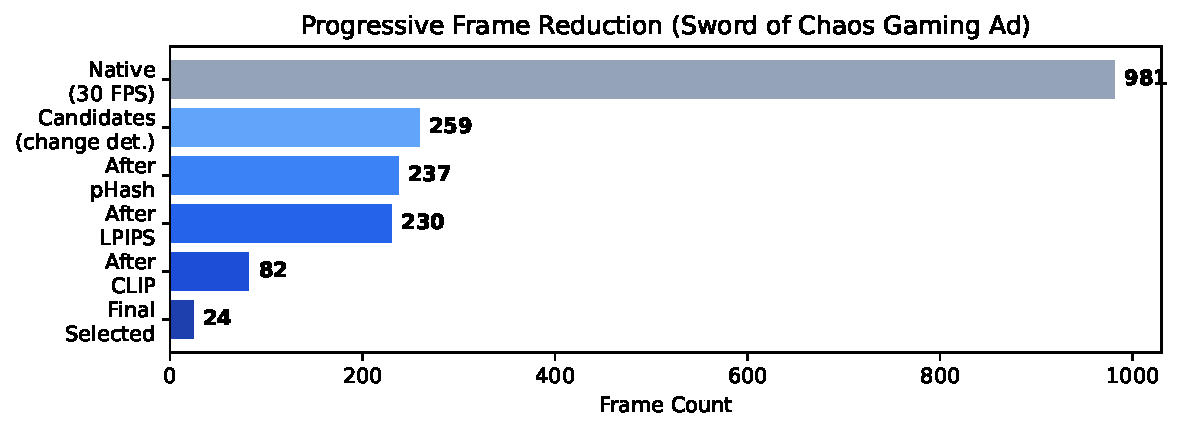
\includegraphics[width=\columnwidth]{Images/cascade_waterfall.pdf}
\caption{Progressive Frame Reduction. Frame counts at each stage of the cascade for the ``Sword of Chaos'' gaming ad (30s at 30 FPS), showing a 97.5\% reduction from native frames to the final VLM input set.}
\label{fig:waterfall}
\end{figure}

\subsubsection{Tier 1: Hash Voting}
For each frame $f_i$, compute three perceptual hashes: pHash~\cite{zauner2010framework} (DCT-based), dHash~\cite{krawczyk2015phash} (gradient-based), and wHash~\cite{wang2019robust} (wavelet-based). Frames are grouped by majority vote: if $\geq 2$ hashes have Hamming distance $< \theta_h$ (default $\theta_h = 10$), frames are considered duplicates. One representative per group advances. This tier eliminates 35\% of frames with $O(1)$ comparison cost.

\subsubsection{Tier 2: Learned Perceptual Similarity}
Remaining frames undergo pairwise LPIPS~\cite{zhang2018unreasonable} comparison:
\begin{equation}
\text{LPIPS}(f_i, f_j) = \sum_l \left\| w_l \odot (\phi_l(f_i) - \phi_l(f_j)) \right\|_2
\end{equation}
where $\phi_l$ are AlexNet layer activations and $w_l$ learned weights. Frames with $\text{LPIPS} < \theta_l$ (default $\theta_l = 0.15$) are merged. This tier handles lighting variations and minor transformations missed by hashes, reducing a further 20\% of frames.

\subsubsection{Tier 3: Semantic Clustering with Temporal NMS}
\label{sec:tanms}
Surviving candidates are embedded via CLIP ViT-B/32~\cite{radford2021learning}. We apply $K$-means clustering with $K = k^*$ from Eq.~\ref{eq:isd}. To prevent temporal clustering (selecting adjacent frames from the same shot), we introduce \textbf{Temporal-Aware NMS (TA-NMS)}:
\begin{equation}
\label{eq:tanms}
f^* = \arg\max_{f \in \text{cluster}_m} \left[ \mathcal{A}(f) - \lambda \cdot \max_{f' \in \mathcal{S}} \exp\left(-\frac{|t_f - t_{f'}|}{\tau_{\text{nms}}}\right) \right]
\end{equation}
where $\mathcal{S}$ is the set of already-selected frames, $\tau_{\text{nms}} = 2.0$\,s controls temporal decay, and $\lambda = 0.3$ balances importance vs.\ diversity. This tier provides the largest single reduction (45\%). 

Figure~\ref{fig:tier_examples} provides empirical examples of frames removed at each tier of the cascade.

\begin{figure*}[t]
\centering
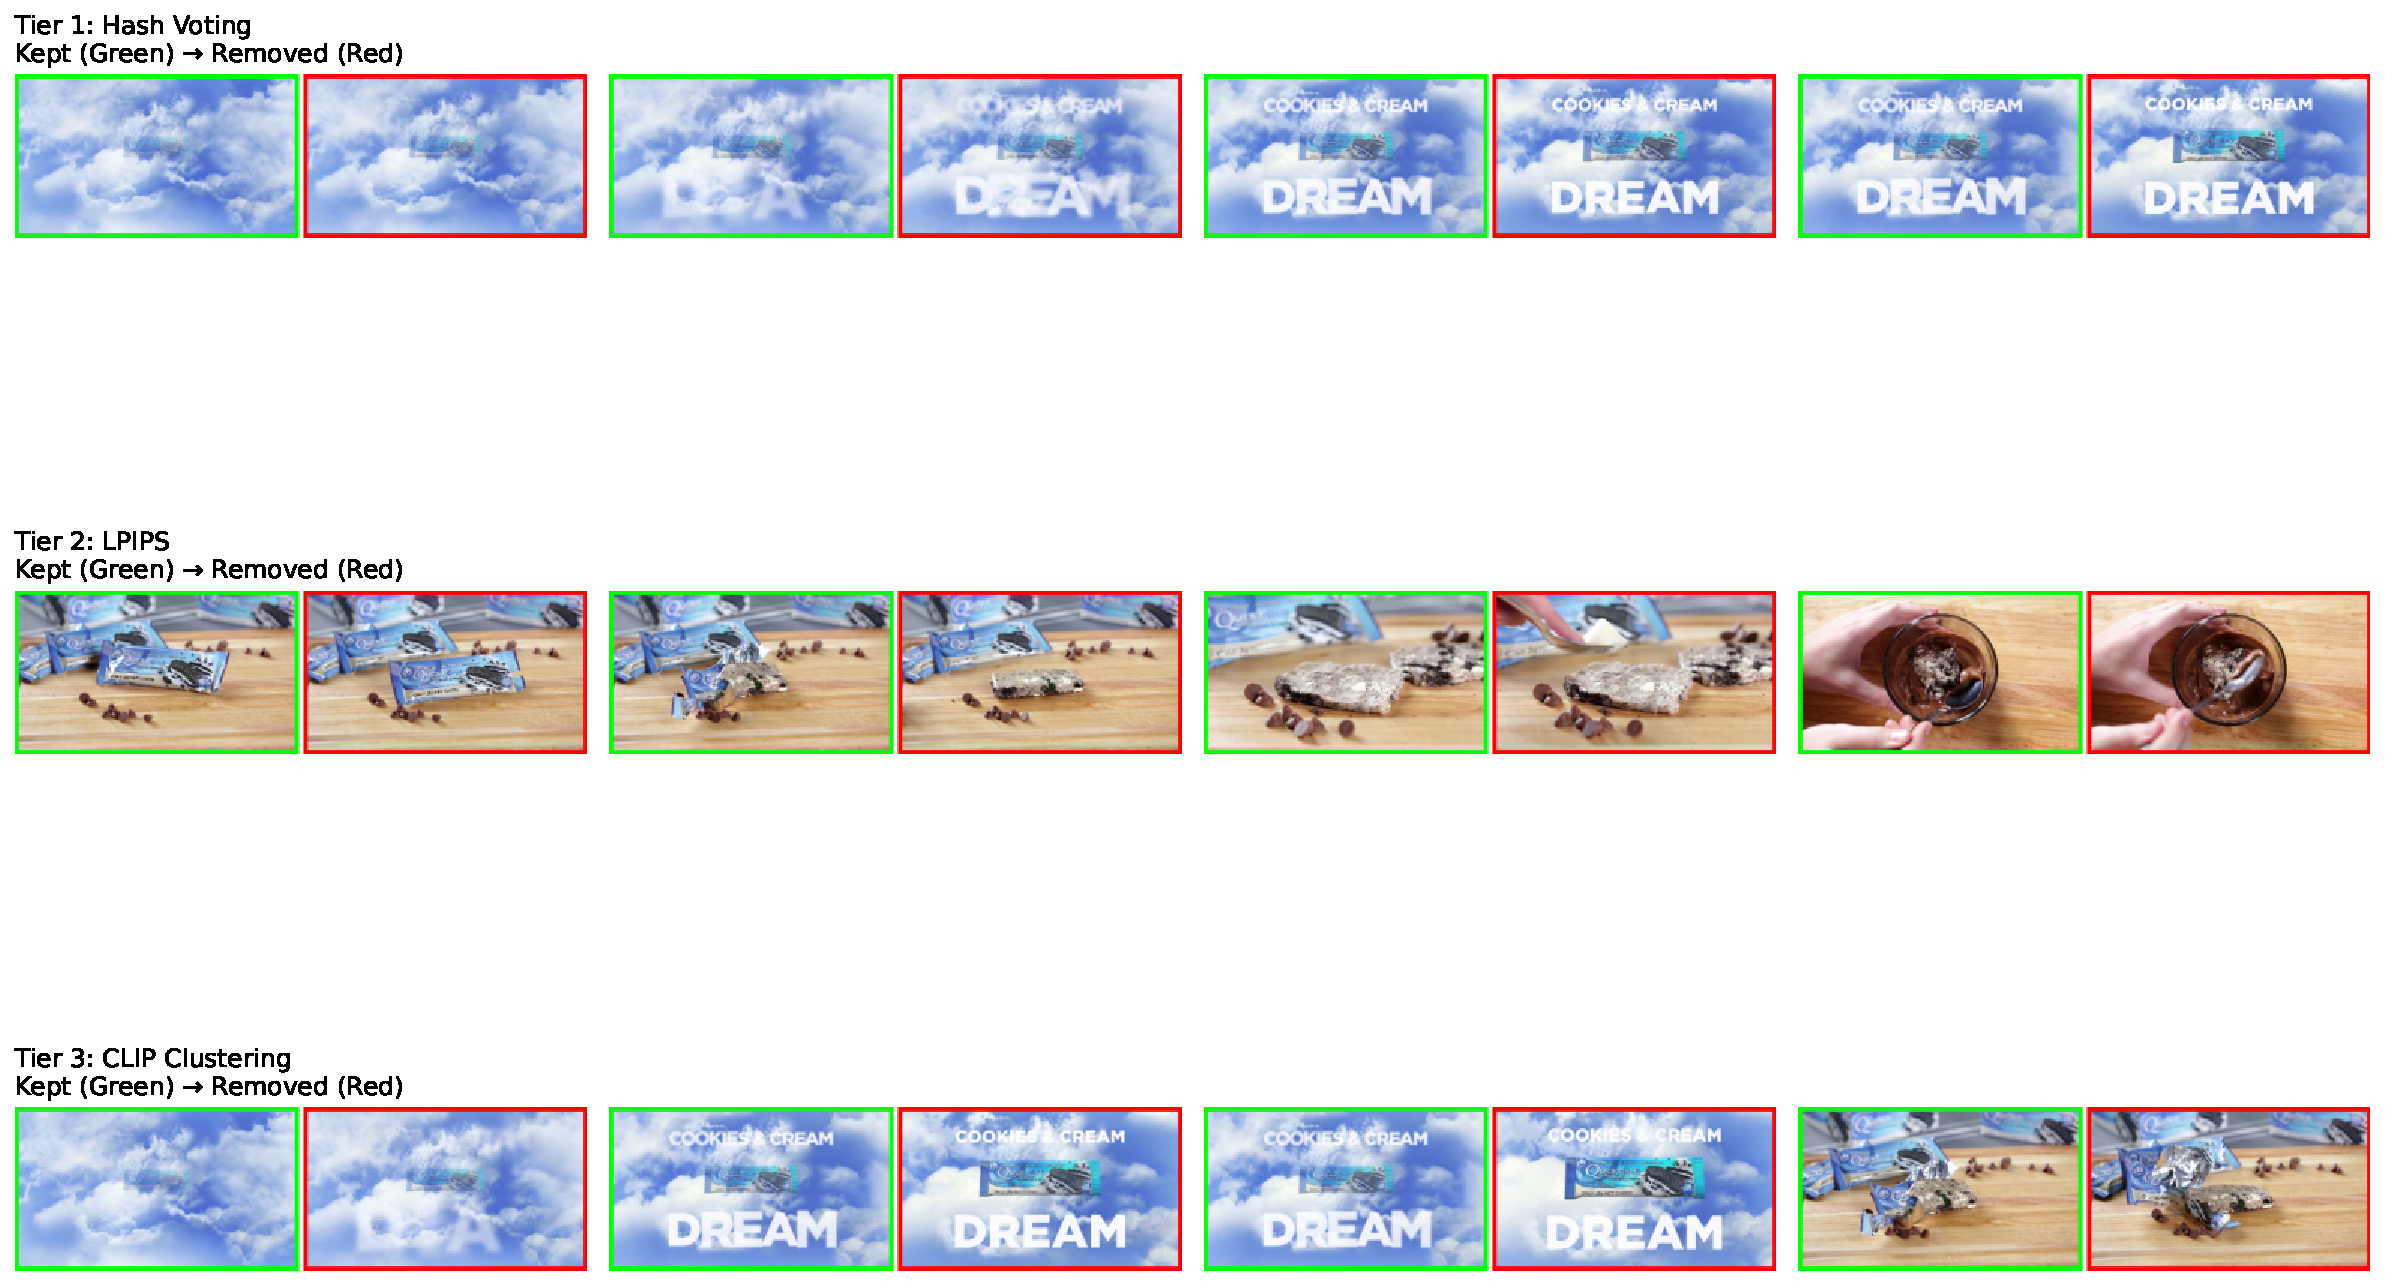
\includegraphics[width=\textwidth]{Images/tier_examples.pdf}
\caption{Per-Tier Deduplication Examples. Tier 1 (Hash Voting) catches identical/near-identical frames; Tier 2 (LPIPS) catches perceptual duplicates across minor transformations; Tier 3 (CLIP) merges semantically redundant shots using cluster-based selection.}
\label{fig:tier_examples}
\end{figure*}

\subsection{Multi-Modal Pipeline Integration}

\textbf{Audio Pipeline}: Whisper-large-v3~\cite{radford2022whisper} transcribes speech. Key phrase detection identifies brand names and product claims. Audio mood classification predicts emotional tone.

\textbf{Visual Pipeline}: Selected frames undergo Tesseract OCR~\cite{smith2007overview} for text extraction. Visual features (text, faces) boost importance scores in TA-NMS.

\textbf{VLM Extraction}: A single prompt queries Gemini-3-Flash for structured JSON output covering: product category, brand names, emotional tone, call-to-action type, visual elements, and target demographic.
